% Created 2013-12-20 金 04:52
\documentclass[12pt]{jsarticle}
\usepackage[dvipdfmx]{graphicx}
\usepackage{comment}
%%\date{\today}
%\title{}
\textheight = 25truecm
\textwidth = 18truecm
\topmargin = -1.5truecm
\oddsidemargin = -1truecm
\evensidemargin = -1truecm
\marginparwidth = -1truecm
\def\theenumii{\Alph{enumii}}
\def\theenumiii{\alph{enumiii}}
\def\labelenumi{(\theenumi)}
\def\labelenumiii{(\theenumiii)}
\begin{document}

%\maketitle
%\tableofcontents

\begin{center}
%%%%%%%%%%%%%%%%%%%%%%%%%%%%%%%%%%%%%%%
%%%タイトル                         %%%
%%%%%%%%%%%%%%%%%%%%%%%%%%%%%%%%%%%%%%%
{\LARGE 「仮想マシンモニタを用いた割り込み処理のデバッグ手法」の要約}
\end{center}

\begin{flushright}
  2014/6/6\\
  藤田将輝
\end{flushright}
%%%%%%%%%%%%%%%%%%1章%%%%%%%%%%%%%%%%%%%
\section{はじめに}
仮想マシンを用いた割り込み処理のデバッグ支援環境の構成を理解するため,情報処理学会研究報告である
「仮想マシンモニタを用いた割り込み処理のデバッグ手法」\cite{doc1}を読解した.
本資料ではこの論文の要約を示す.

\section{目的}
OSの複雑化,多機能化に伴い,OS内部に存在するバグが増えている.
このため,OSのデバッグが重要になっている.
OSのデバッグは困難であり,その理由の一つに非同期処理である,割り込みの再現がある.
非同期処理とはデータを転送する際に,送信側と受信側のタイミングの一致を気にせずにデータをやり取りする処理である.
割り込み処理は非同期的に発生し,常に同じタイミングで発生するとは限らないため,再現が難しい.
本研究では割り込みのタイミングを制御可能にすることでOSのデバッグを支援する手法を提案する.
提案手法では仮想マシンモニタを利用し,割り込みのタイミングを制御する.
\section{割り込み}
割り込みは,どのタイミングでどの割り込みが発生しても正しく処理しなければならない.
まず,割り込みは適切に禁止/許可されなければならない.
割り込みが発生することにより,処理結果に影響を受ける関数や,プログラムがあるためである.
また,どのようなデータを受け取っても適切に処理しなければならない.
受け取ったデータがどのようなものでもデータ構造を壊したり,NULLポインタを参照したりしてはならないためである.

\section{提案手法}
\subsection{概要}
提案手法では使用者が割り込みを発生させるコード位置と割り込みの種類を指定する.
指定したコード位置で任意の割り込みを発生させる.
この手法を用いることで,任意のタイミングで任意の種類の割り込みを意図的に発生させることができる.
\subsection{割り込み挿入の方法}
提案手法を実現するために,仮想マシンモニタ(VMM)による仮想環境を用いる.
仮想環境では仮想マシンのイベントをVMMがエミュレートする.
エミュレートとは仮想マシンの動きを再現することである.
提案手法ではデバッグ対象OSをゲストOSとして動作させる.
VMMを用いることで意図的にゲストOSに割り込みを発生させることができる.
提案手法における割り込み処理の流れを図1に示し,以下で説明する.
\begin{enumerate}
\item デバッグ対象OSの割り込みを挿入したいコード位置にtrapを発生させるコードを挿入し,ゲストOSとして動作させる.
なお,trapには割り込みの種類とデータを指定しておく.
\item (1)で指定したコード位置でゲストOSがtrapを発生する.
\item VMMがホストOSへ割り込みデータを準備するリクエストを渡す.
\item ホストOSが割り込みデータを作成し,VMMにデータ作成完了を通知する.
\item VMMがゲストのCPUの状態を書き換える.なお,ゲストOSのCPUの状態はVMCSというデータ領域で管理されており,
実際にはこれを書き換える.
\item 処理がゲストOSに移り,CPUがデータ領域を参照し,割り込みが挿入される.
\end{enumerate}
これにより,指定したコード位置に割り込みを挿入させることができる.

\begin{figure}[t]
\begin{center}
\includegraphics[height=5.5cm]{./fig3.jpg}          
\caption{提案手法における割り込み処理の流れ}
\label{fig:up}
\end{center}
\end{figure}


\section{実装}
\subsection{概要}
提案手法を仮想マシンモニタXen4.1.0に実装した.
XenではゲストOSをdomU,ホストOSをdom0と呼ぶ.
提案手法の実装イメージを図2に示し,以下で説明する.
\begin{enumerate}
\item domUの割り込みを発生させるコード位置にhypercallを挿入する.
\item 挿入したhypercallがtrapを生成する.
\item Xenがdom0に割り込みデータ作成のリクエストを渡し,dom0がデータを作成する.
\item dom0はXenに割り込みデータ作成完了を通知する.
\item XenがVMCSを書き換える.
\item CPUがVMCSを参照し,割り込みを挿入することで,domUで仮想的に割り込みが発生する.
\end{enumerate}
Xenでは,割り込みデータをqemu-dmで処理している.
そこで,qemu-dmに変更を加え,データを準備する機構を作成する.

\begin{figure}[t]
\begin{center}
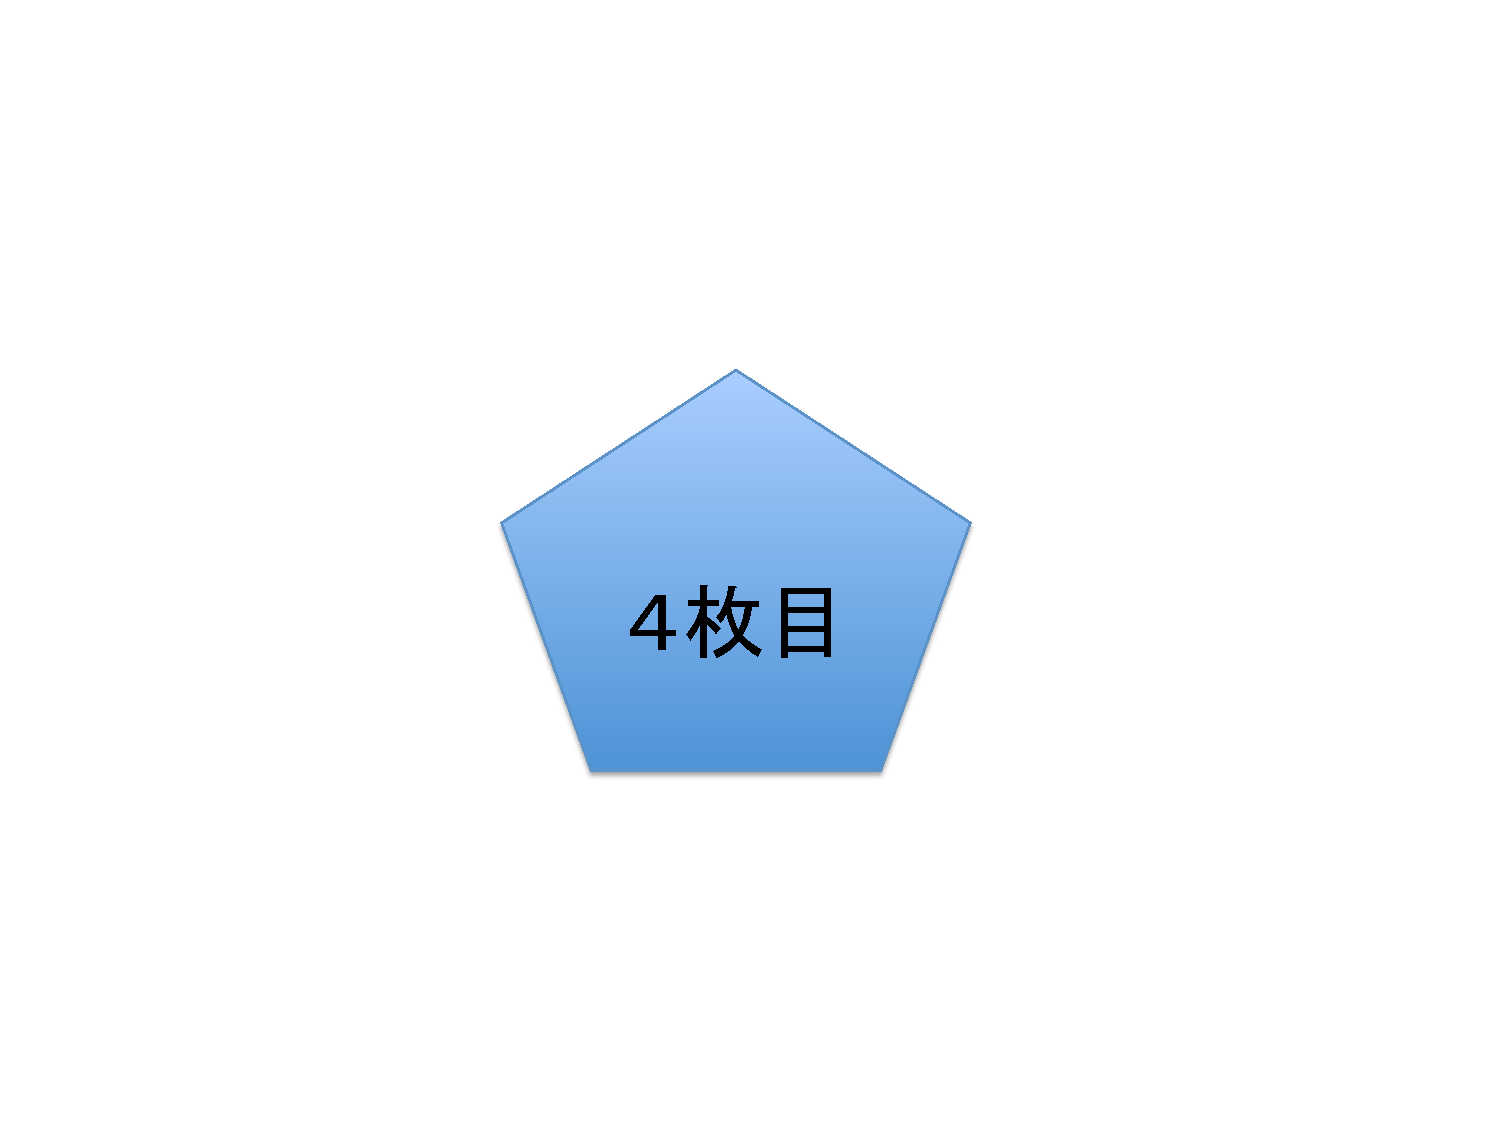
\includegraphics[height=5.5cm]{./fig4.jpg}          
\caption{実装図}
\label{fig:up}
\end{center}
\end{figure}


\subsection{割り込み挿入位置の指定}
ゲストOSの割り込みを挿入させたいコード位置にハイパーコールであるVMCALLを挿入する.
VMCALLはレジスタの中身を引数として渡すことができ,割り込みの種類を指定する.
また,送信する割り込みデータもここで指定する.
\subsection{割り込みの挿入}
割り込みの挿入はXenがVMCSを書き換えることで行う.
具体的にはVMCSのVM-entry control fieldという領域における,
VMEntry Controls for Event Injectionという領域を書き換える.
これにより,VMMからdomUに処理が移る際に割込みを仮想的に挿入できる.
dom0がリクエストを受けてから割り込み挿入までの流れを以下に示す.
\begin{enumerate}
\item dom0がデータを準備するリクエストを受け取り,割り込みデータをエミュレート
する関数を呼び出す.
\item 割り込みデータをエミュレートする関数により,割り込みデータをdomUのドライバ用のデータに変更する.
\item 関数の処理が完了すると,Xenに割り込みデータの作成完了を通知する.
\item Xenが,通知を受け取り,VMCSを書き換え,操作をdomUに移す.
\item 操作が移る際,CPUがVMCSを参照し,仮想的に割り込みが発生する.
\end{enumerate}
\section{まとめ}
本研究では割り込みのタイミングを意図的に制御可能にすることによりデバッグを支援する手法を提案した.
また,Xen4.1.0上に割り込みを意図的に挿入する機構を作成した.
domU の検査対象コードから呼び出されるハイパー
コールをうけ,XenがVMCSを書き換える仕組みを実装
した.また,qemu-dm上に,割込みのデータを準備する機
構を作成した.
この機構を利用してタイマ割り込み,キーボード割り込み,ネットワーク割り込みの挿入を行えるようにした.
現在挿入できている割り込みは,タイマ割り込み,キーボード割り込み,ネットワーク割り込みのみである.
これ以外の割り込みについては対応できていない.
また,現在の実装ではハイパーコールをコードに直接埋め込んでいるため,利用者が入れるべき割り込み場所,
種類を予想して利用しなければならない.

\section{おわりに}
本資料では「仮想マシンモニタを用いた割り込み処理のデバッグ手法」\cite{doc1}を要約した.
仮想マシンを用いたデバッグ支援手法の目的と動きを理解した.
また,割り込みにおけるバグの例を知ることができた.
仮想化を用いた割り込みのデバッグ環境とMintを用いたデバッグ支援機構と照らし合わせ,デバッグ支援機構の理解を深める.

\begin{thebibliography}{9}
\bibitem{doc1} 宮原俊介,吉村剛,山田浩史,河野健二:仮想マシンモニタを用いた割り込み処理のデバッグ手法,情報処理学会研究報告,Vol.2013-OS-124,No.6,pp.1-8(2013)
\end{thebibliography}

\end{document}
